\documentclass[12pt, a4paper]{article}
\usepackage[margin = 1in, top=1.3in]{geometry}
\usepackage[english]{babel}
\usepackage[utf8]{inputenc}
\usepackage{fancyhdr}
\usepackage{amsmath}
\usepackage{bm}
\usepackage{graphicx}
\graphicspath{{./images/}}
\usepackage[font=small,labelfont=bf]{caption}
 
\pagestyle{fancy}
\fancyhf{}
\rhead{\small{Niraj Mahajan (180050069)\\ Raaghav Raaj (180050082)}}
\lhead{CS-215 Assignment-4 : Question 5}
\rfoot{Page 5.\thepage}
 
\begin{document}
\section*{Question 5}
\subsection*{5.1 : Part A}
\hspace{1cm} For the collection of images, the Mean Vectors, Covariance Matrices, eigenvalues, and corresponding eigenvectors have been calculated and stored in 'results.mat' (present in the results directory). More on it's loading in Sub-Section 5.4 (Usage of code). The mean and the first four eigenvectors have also been plotted, and the plots follow:

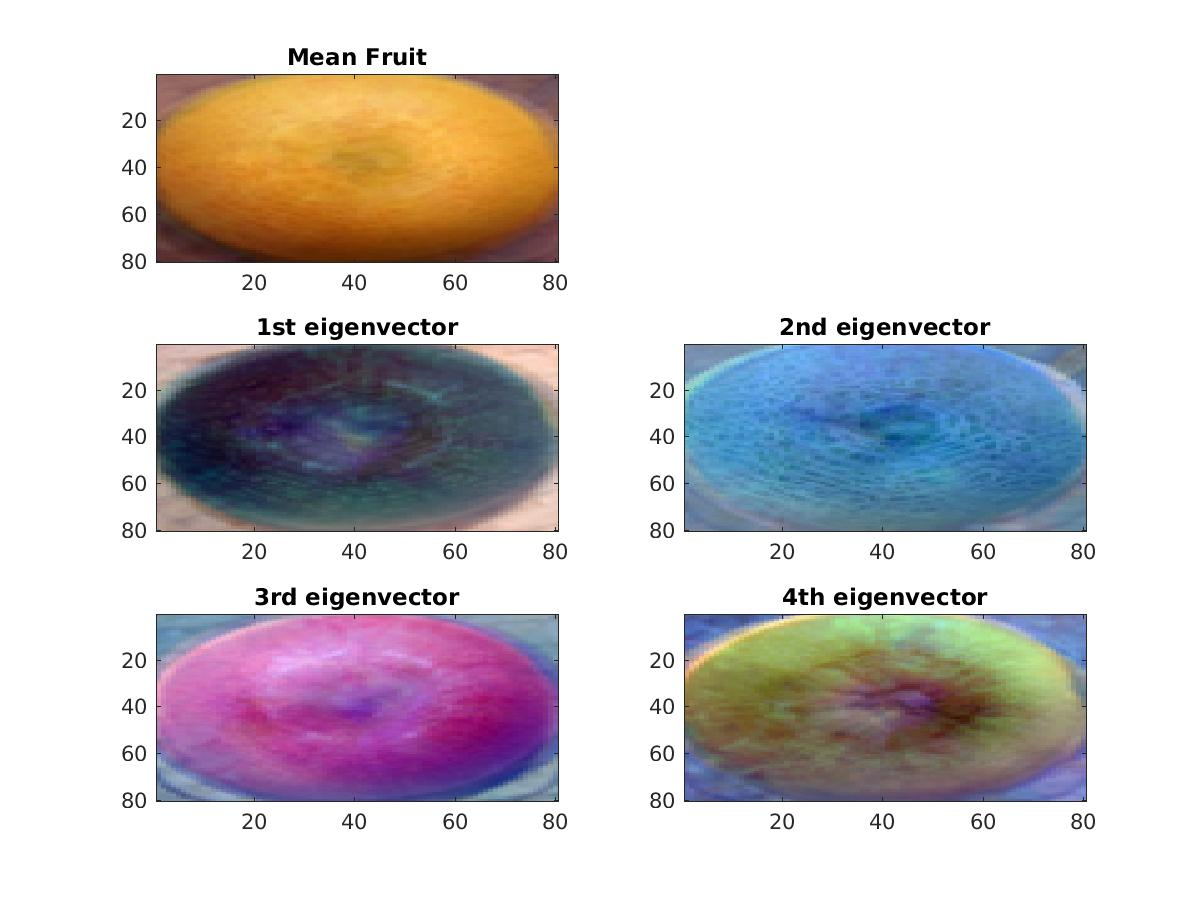
\includegraphics[width=\textwidth, height = 0.6\paperheight]{Mean_and_4Eigen}
\begin{minipage}{\linewidth}
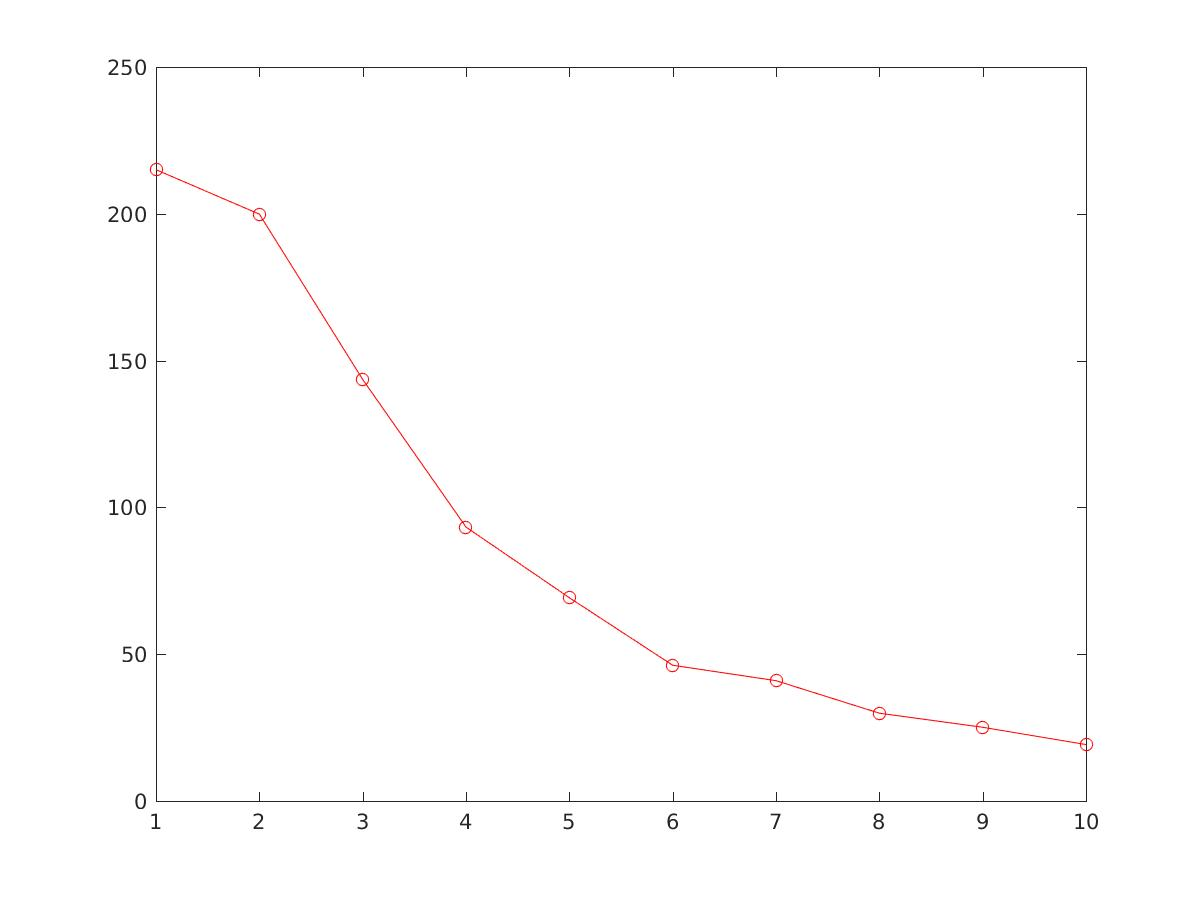
\includegraphics[width=\textwidth, height = 0.4\paperheight]{Eigen10}
\captionof{figure}{Plot of Largest 10 eigenValues vs components}
\end{minipage}


\subsection*{5.2 : Part B}
\hspace{1cm} We have been given 16 images to train, with each image having 80x80x3 = 19200 variables. Let us call each of these images an instance. Let us denote a general variable as follows:
$$X_i^j = i^{th} \; variable \; of \; the \; j^{th} \; image \; instance$$
\vspace{-30pt}
\begin{flushright}
$\forall \;\; i \leq 19200, \; \; j \leq 16$
\end{flushright}
Let our eigenvectors corresponding to the top 4 eigenvalues be $\mathbf{V_1}$, $\mathbf{V_2}$, $\mathbf{V_3}$ and $\mathbf{V_4}$. \\
Let the mean Vector over all fruits be $\boldsymbol{\mu}$ and let $\mathbf{X^i}$ be a 19200x1 vector of the ith image instance.\\ \\
Note that all four eigenvectors have zero inner product with respect to each other, since the Covariance matrix is SPD (Symetric Positive Definite)\\ \\
Hence $\forall \; i \leq 16, \; a_i \; \in \; R^+ $
\begin{align*}
\boldsymbol{X^i} &= \boldsymbol{\mu} + a_1\boldsymbol{V_1} + a_2\boldsymbol{V_2} + a_3\boldsymbol{V_3} + a_4\boldsymbol{V_4}
\end{align*}
We are keeping the coefficient of $\boldsymbol\mu$ as 1, since it is the mean matrix.\\
Multiplying the equation with the transpose of each eigenvector, since their inner product is zero.
\begin{align*}
\boldsymbol{X^i} &= \boldsymbol{\mu} + \sum_{i=0}^4 a_i\boldsymbol{V_i} \\
\boldsymbol{X^i.V_j^T} &= \boldsymbol{\mu.V_j^T} + \sum_{i=0}^4 a_i\boldsymbol{V_i.V_j^T} \\
\boldsymbol{X^i.V_j^T} &= \boldsymbol{\mu.V_j^T} + \sum_{i \neq j} a_i\boldsymbol{V_i.V_j^T} + a_j<\boldsymbol{V_j, V_j}>\\
a_j &= \frac{\boldsymbol{X^i.V_j^T} - \boldsymbol{\mu.V_j^T}}{<\boldsymbol{V_j, V_j}>} \;\;\;\;\;\; \forall j \in \{1,2,3,4\}\\
\end{align*}
Hence we can find the closest representation of every fruit as a linear combination of the mean and the first four eigen vectors.\\
The fruits, along with their closest representation follow:

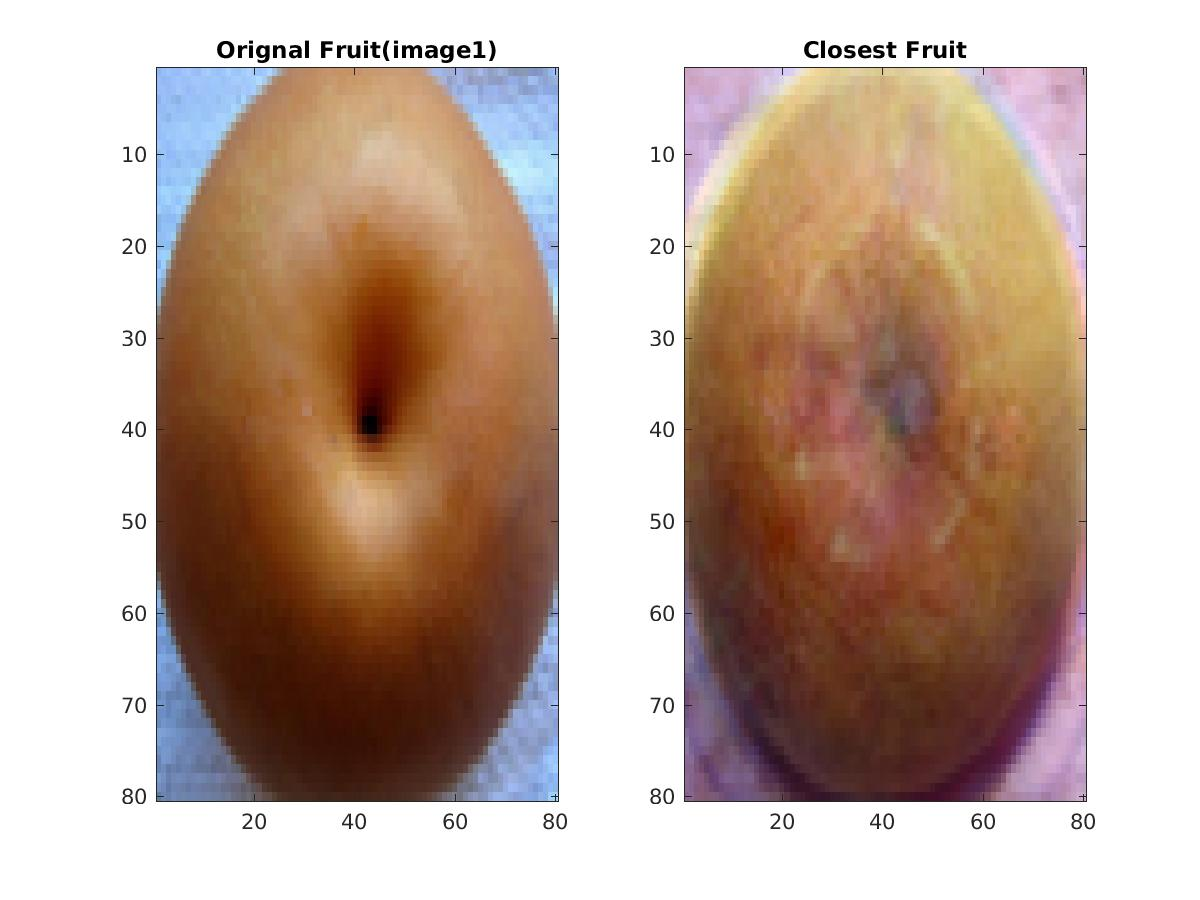
\includegraphics[width=\textwidth, height = 0.25\paperheight]{Closest_fruit_analysis_1}
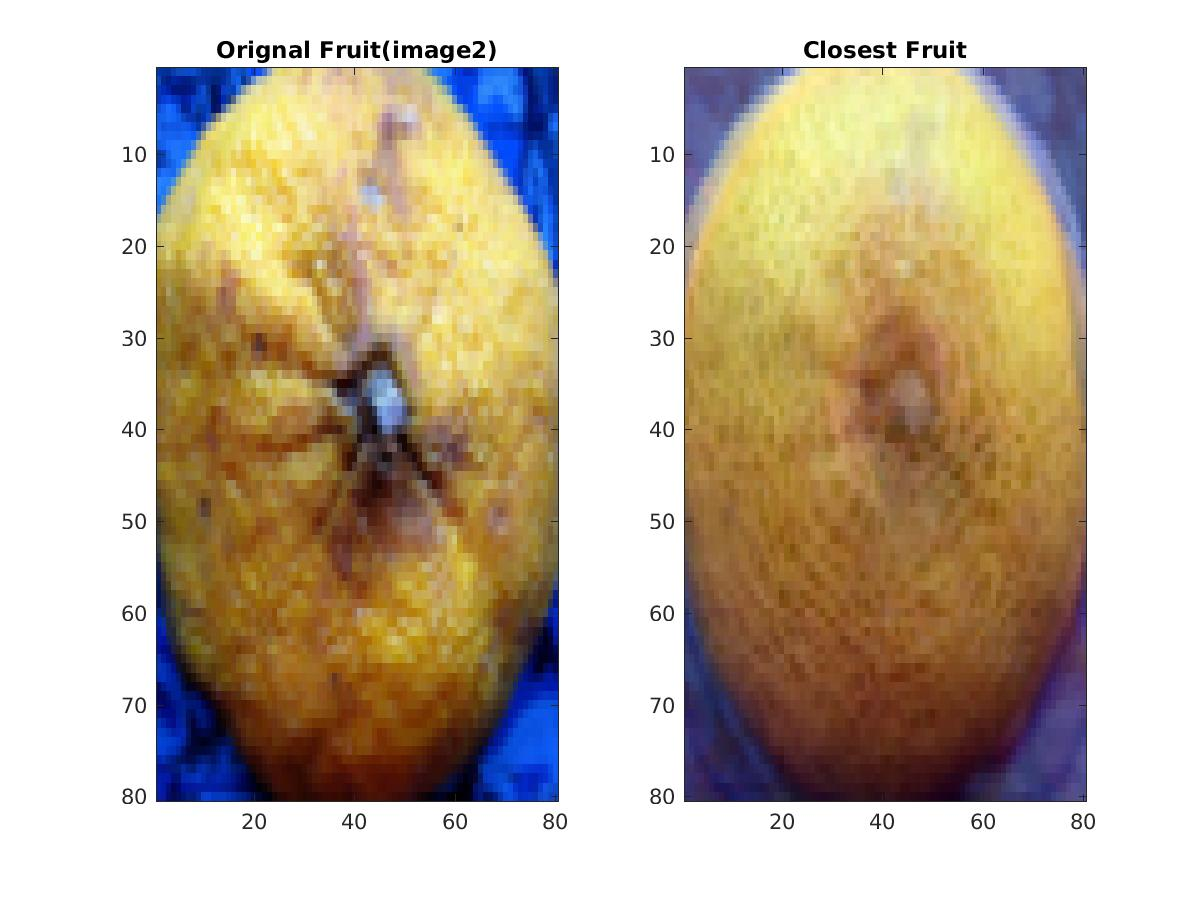
\includegraphics[width=\textwidth, height = 0.25\paperheight]{Closest_fruit_analysis_2}
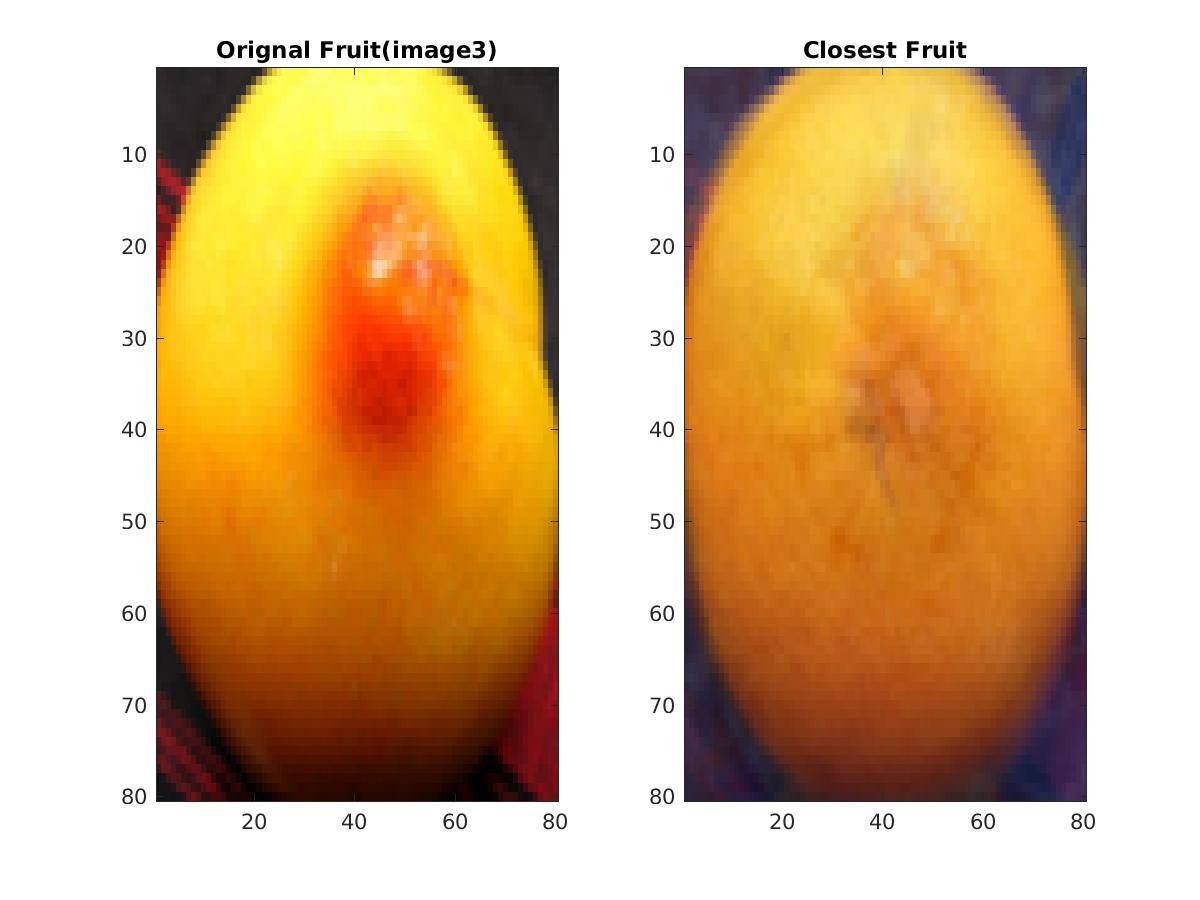
\includegraphics[width=\textwidth, height = 0.25\paperheight]{Closest_fruit_analysis_3}
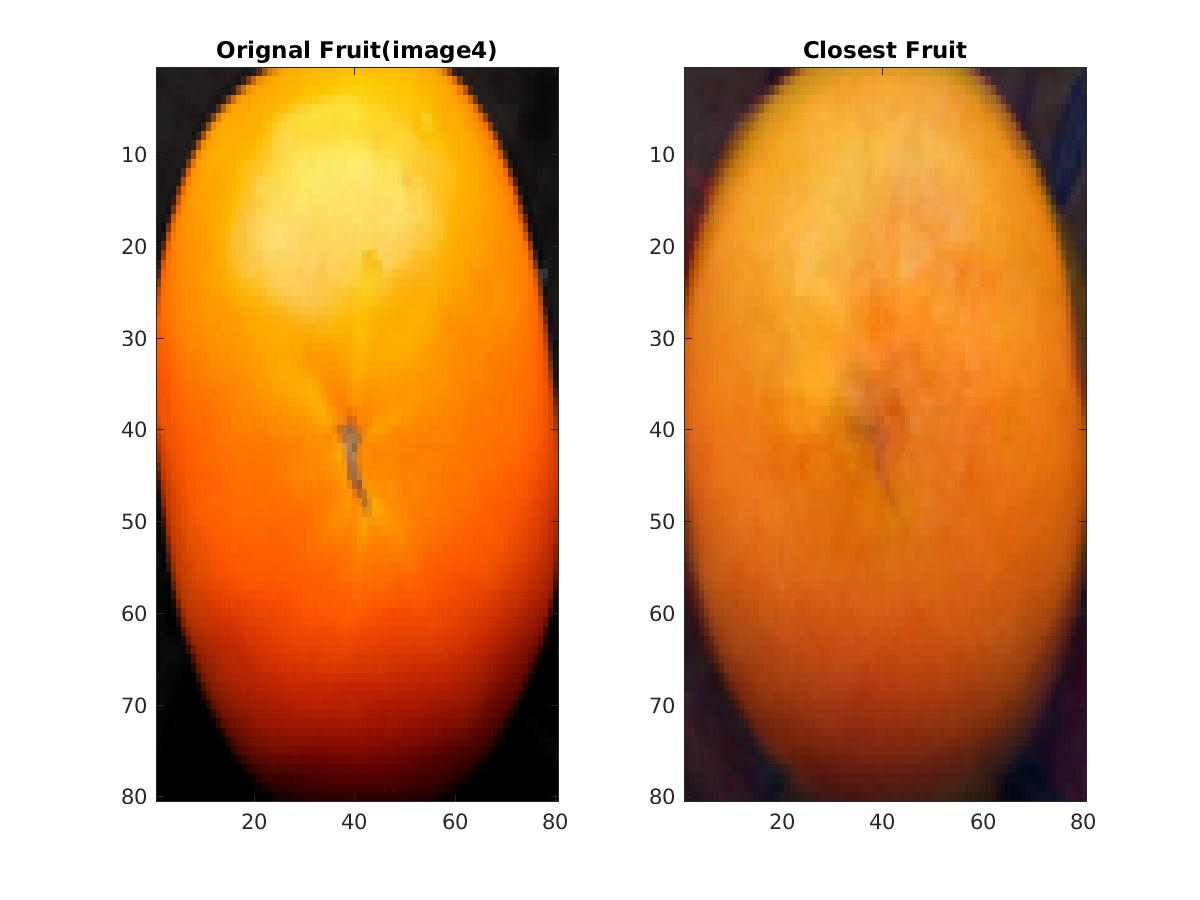
\includegraphics[width=\textwidth, height = 0.25\paperheight]{Closest_fruit_analysis_4}
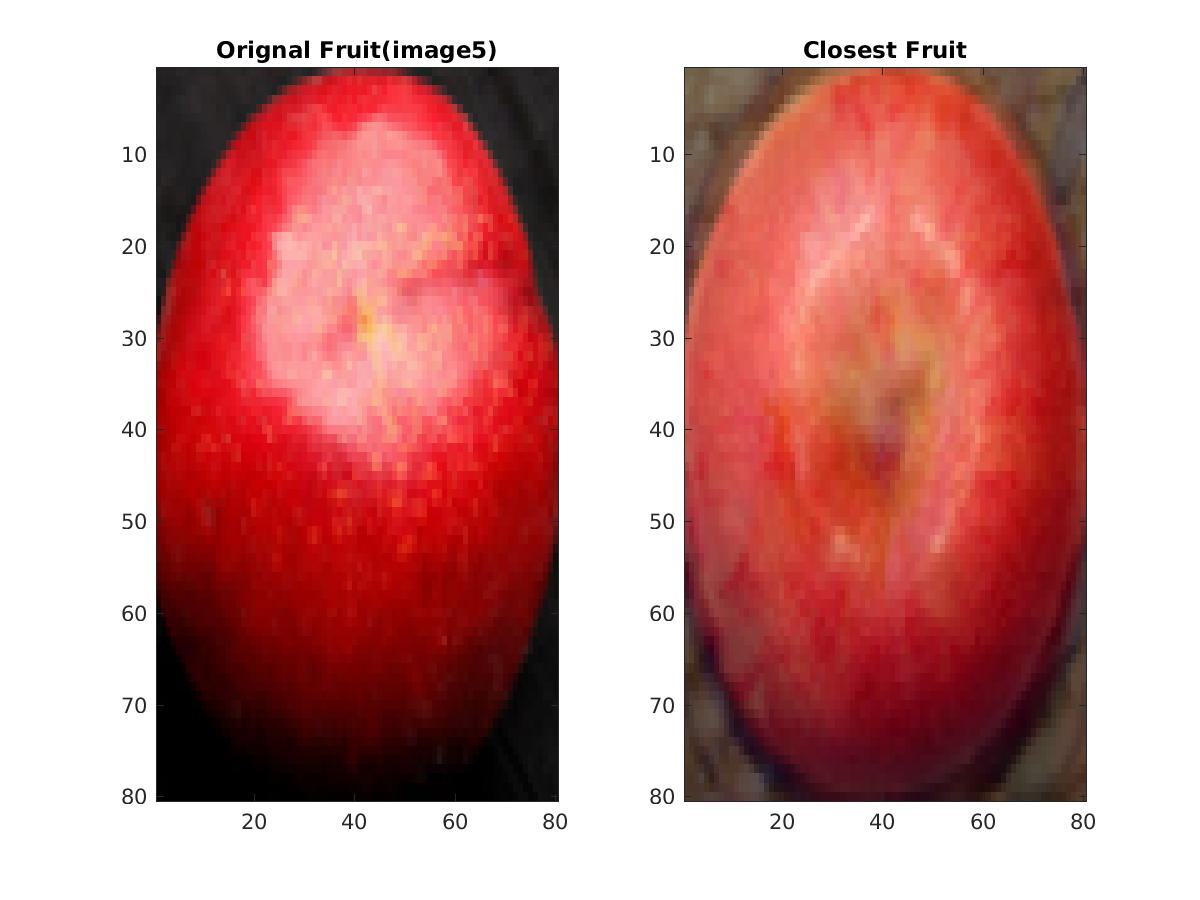
\includegraphics[width=\textwidth, height = 0.25\paperheight]{Closest_fruit_analysis_5}
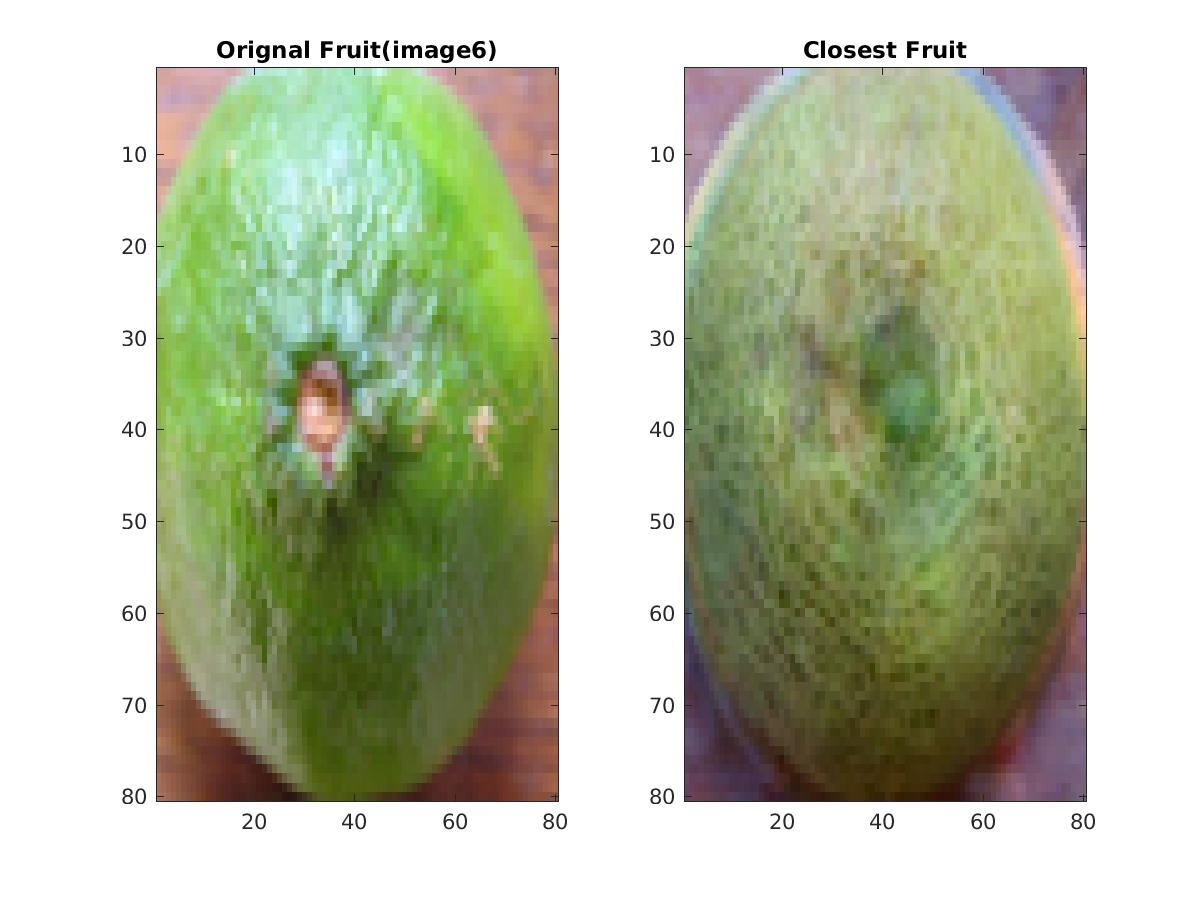
\includegraphics[width=\textwidth, height = 0.25\paperheight]{Closest_fruit_analysis_6}
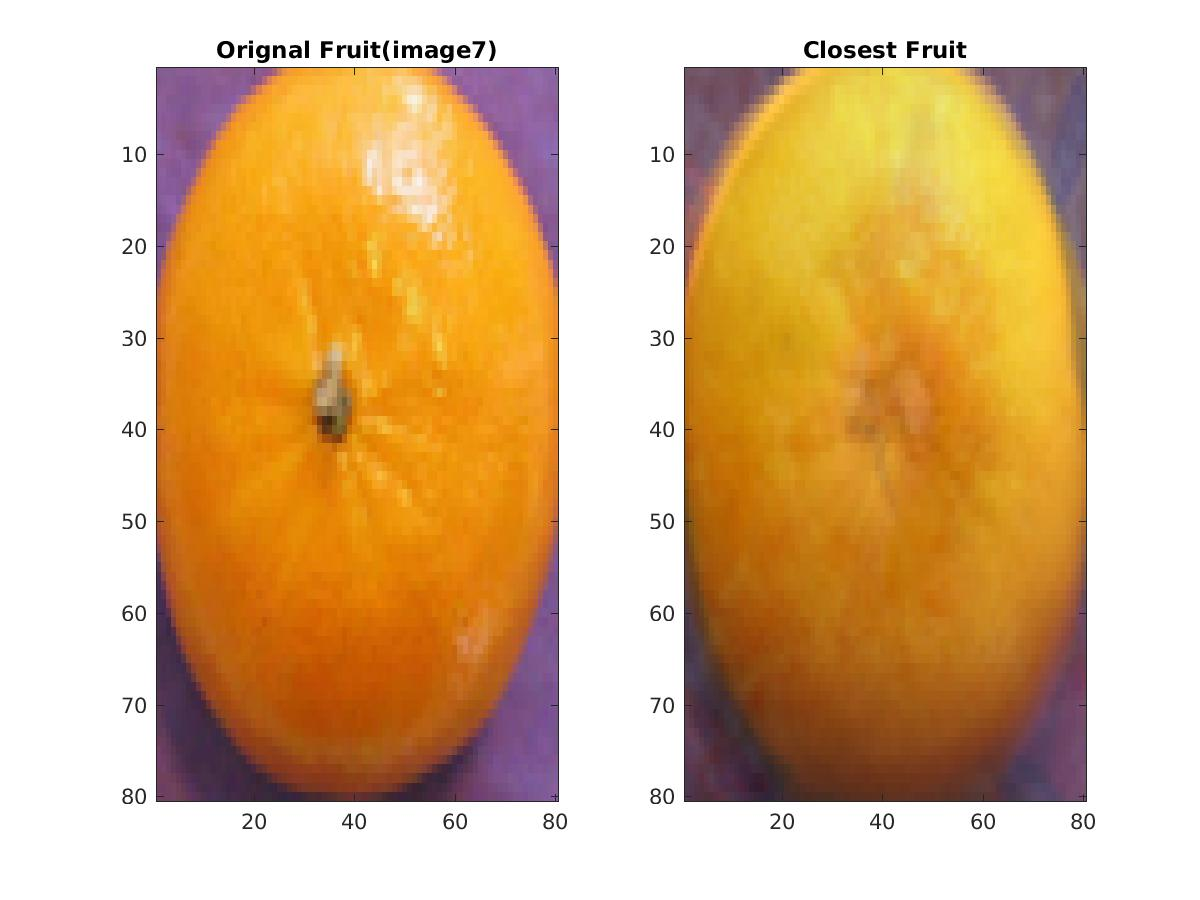
\includegraphics[width=\textwidth, height = 0.25\paperheight]{Closest_fruit_analysis_7}
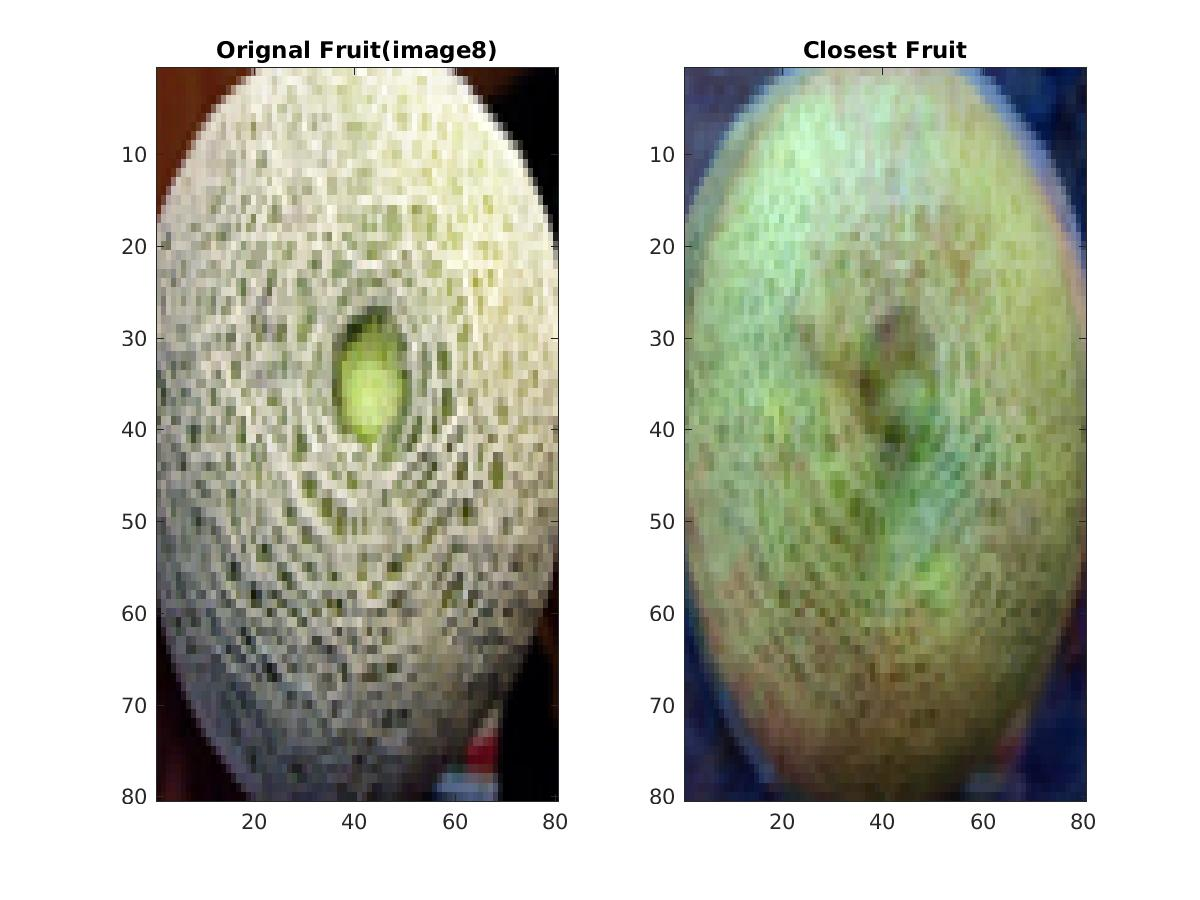
\includegraphics[width=\textwidth, height = 0.25\paperheight]{Closest_fruit_analysis_8}
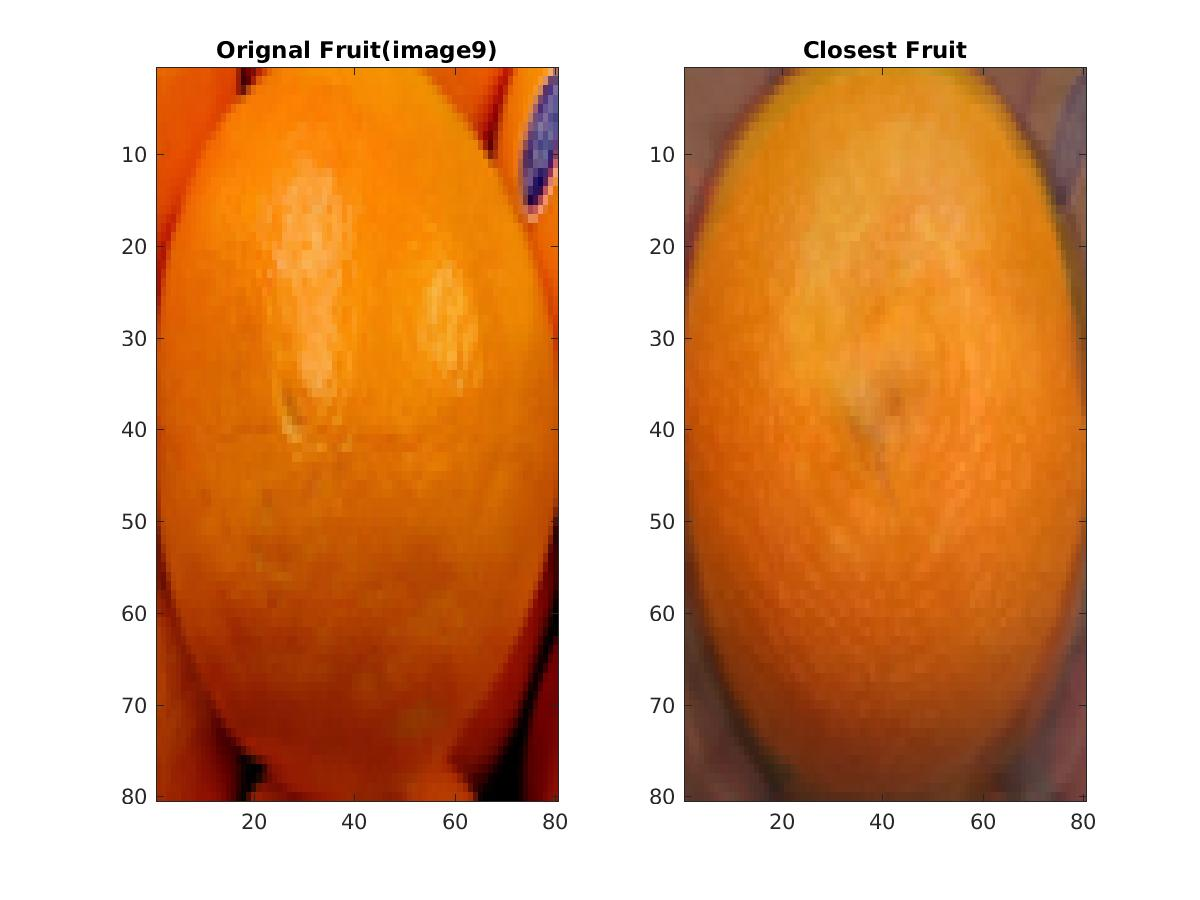
\includegraphics[width=\textwidth, height = 0.25\paperheight]{Closest_fruit_analysis_9}
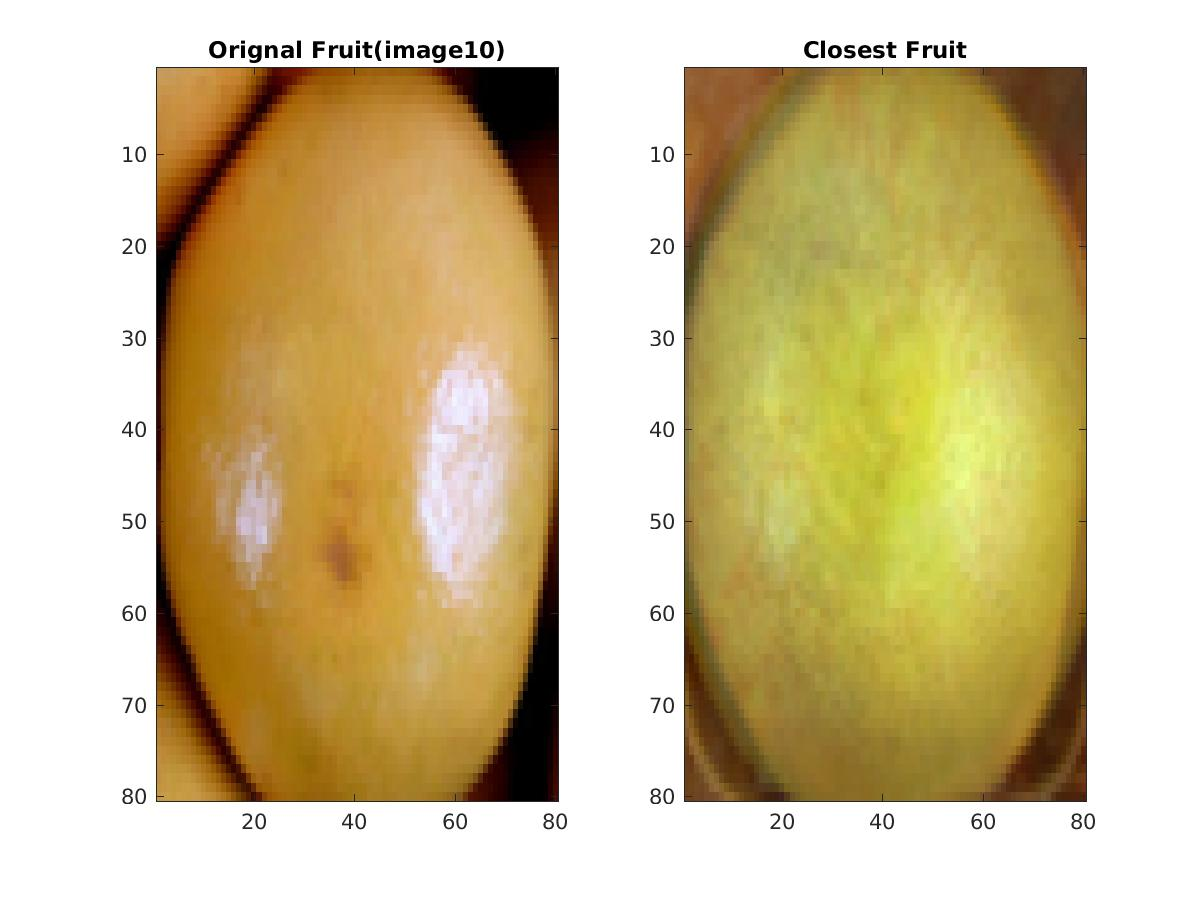
\includegraphics[width=\textwidth, height = 0.25\paperheight]{Closest_fruit_analysis_10}
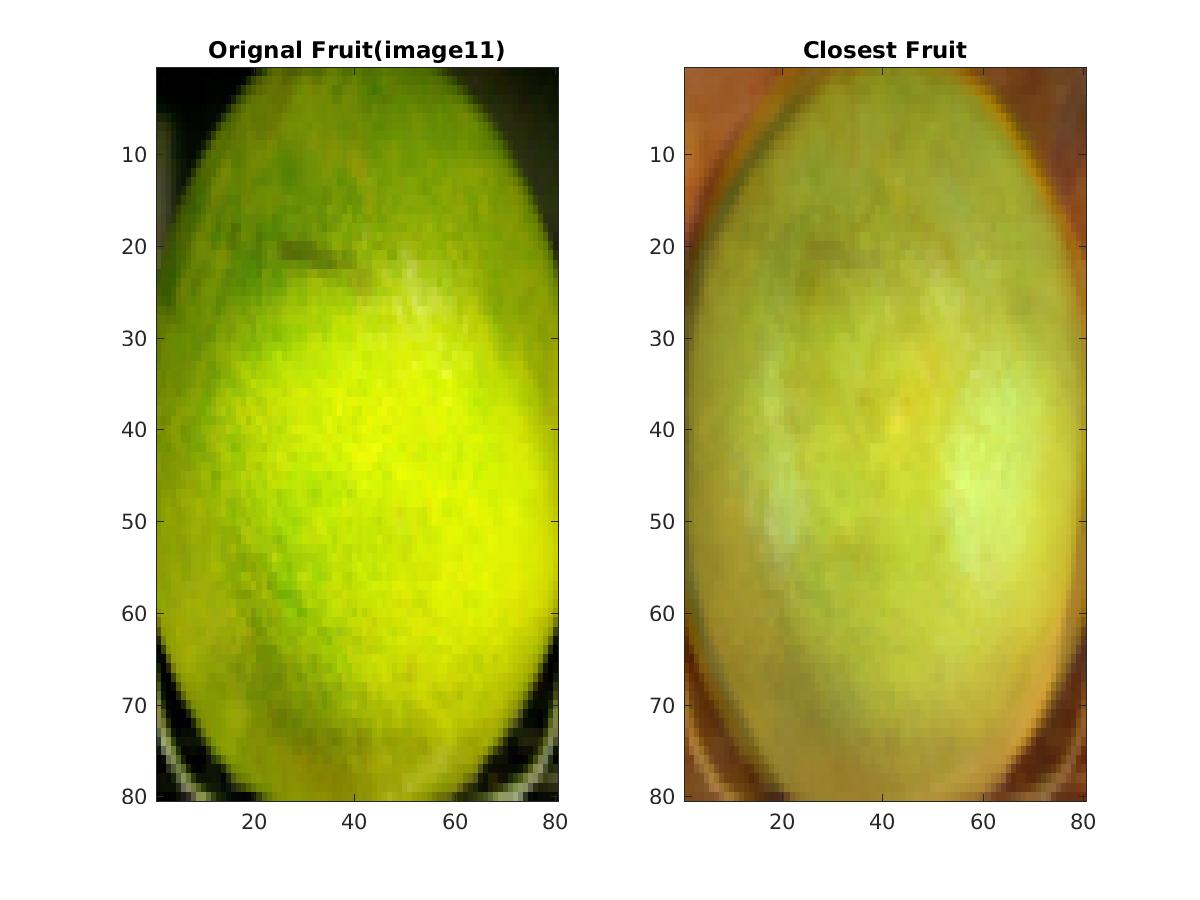
\includegraphics[width=\textwidth, height = 0.25\paperheight]{Closest_fruit_analysis_11}
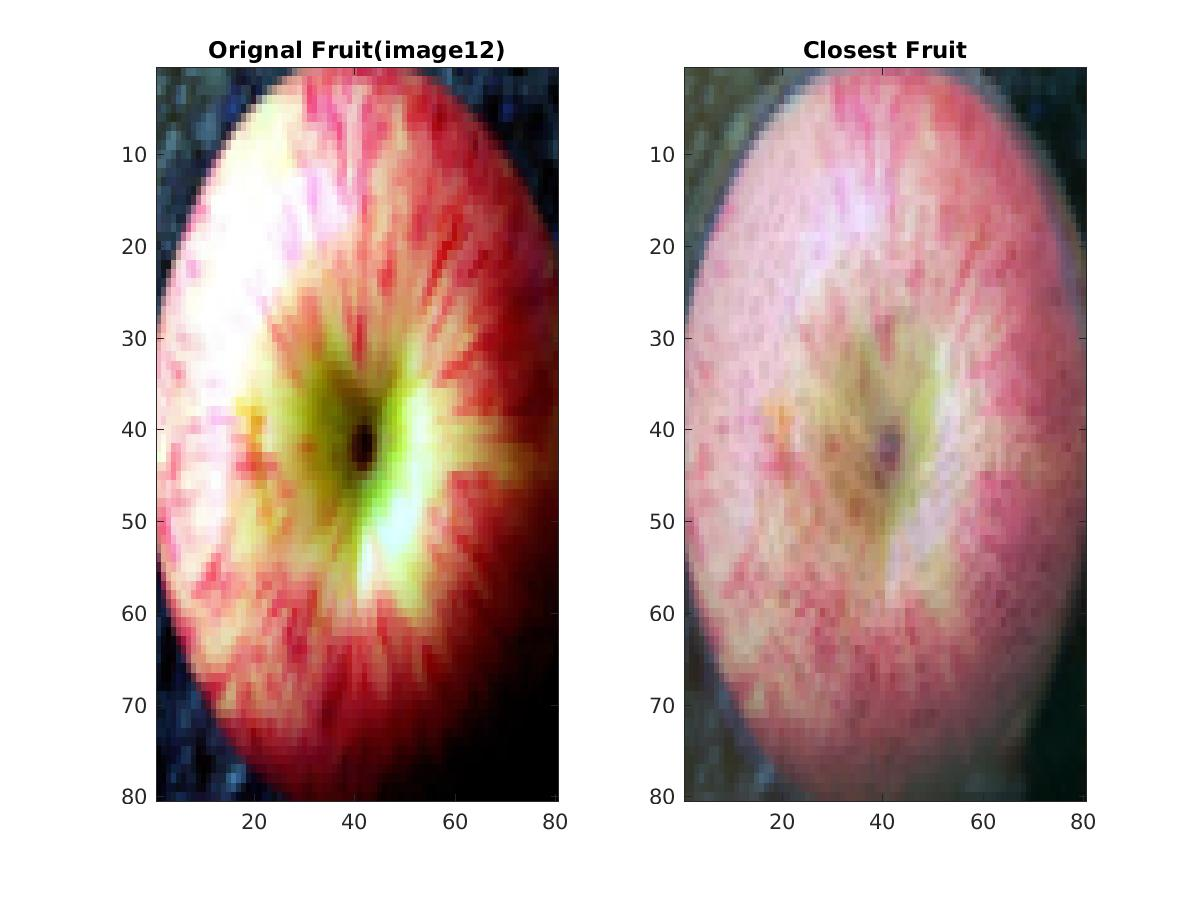
\includegraphics[width=\textwidth, height = 0.25\paperheight]{Closest_fruit_analysis_12}
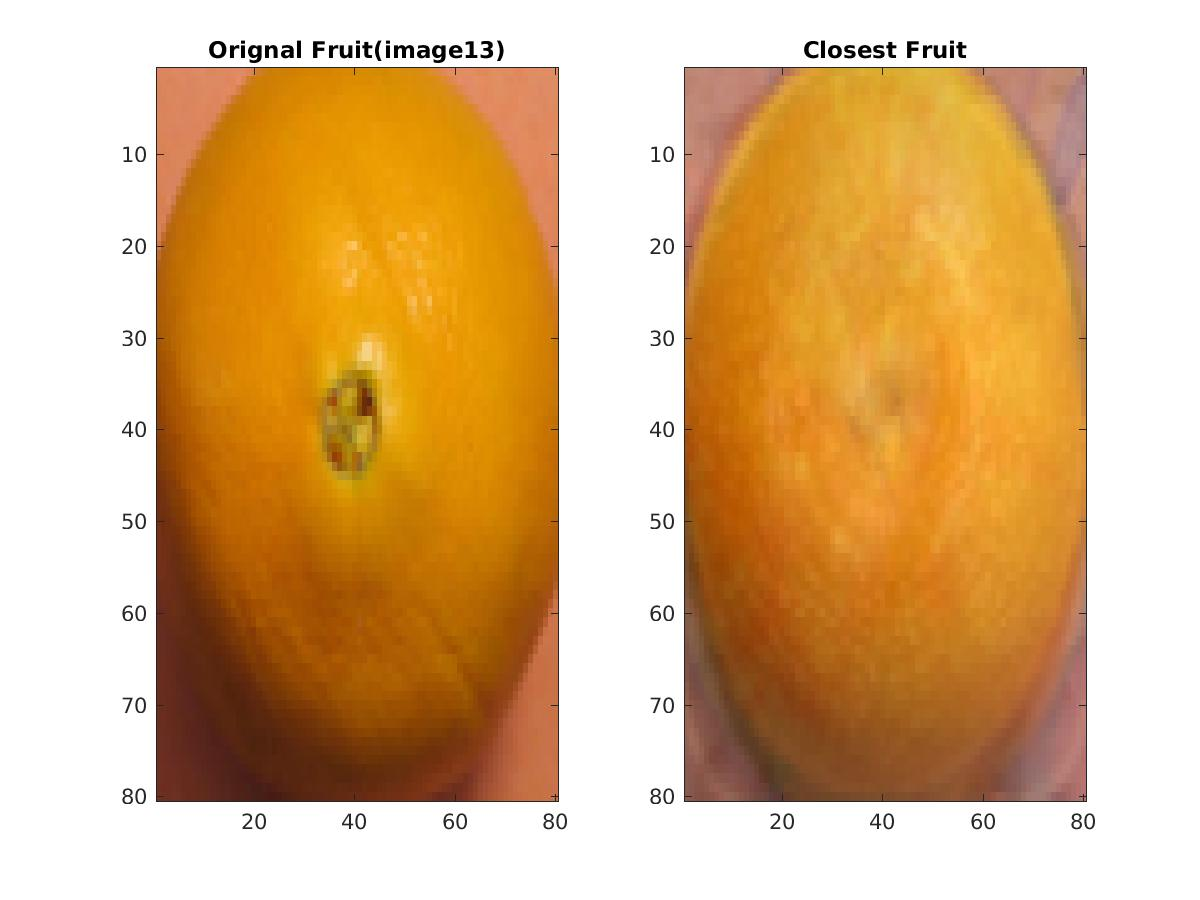
\includegraphics[width=\textwidth, height = 0.25\paperheight]{Closest_fruit_analysis_13}
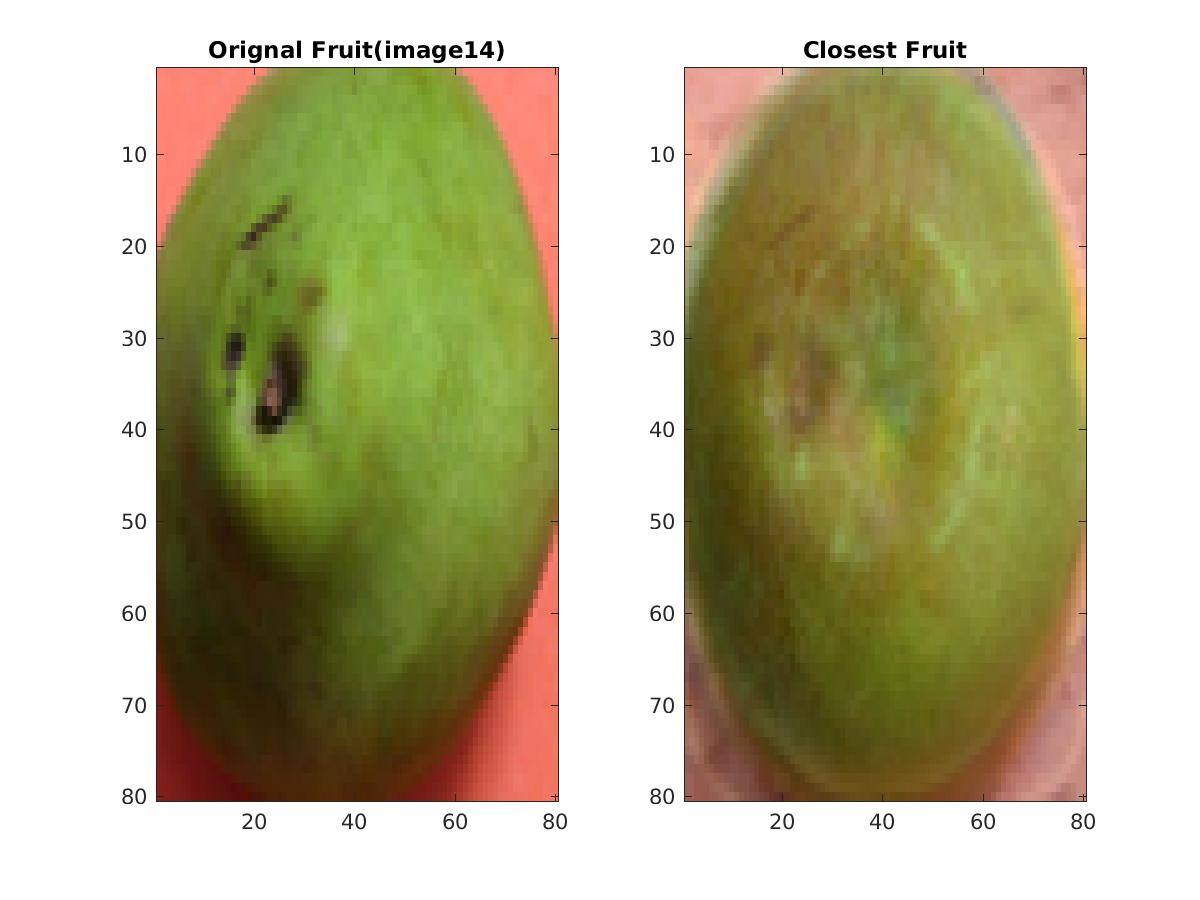
\includegraphics[width=\textwidth, height = 0.25\paperheight]{Closest_fruit_analysis_14}
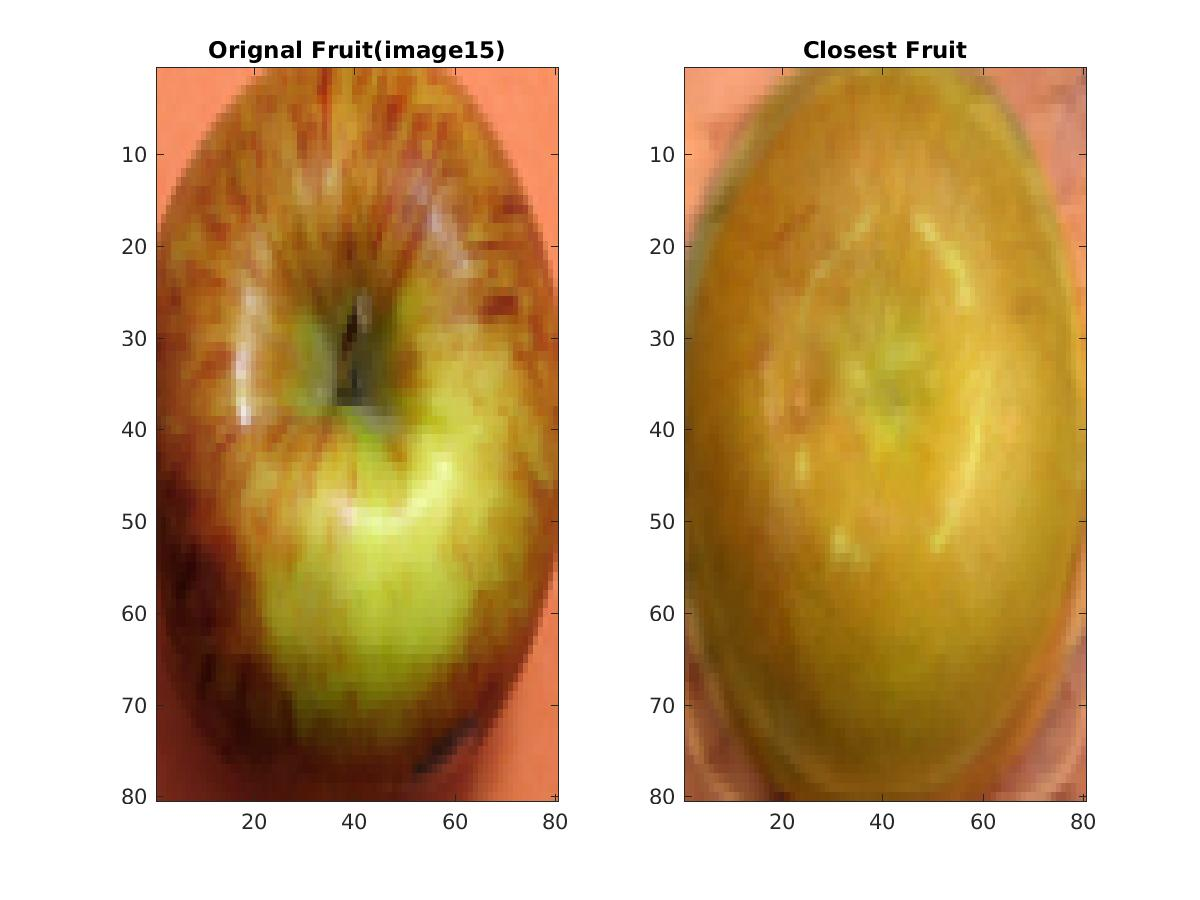
\includegraphics[width=\textwidth, height = 0.25\paperheight]{Closest_fruit_analysis_15}
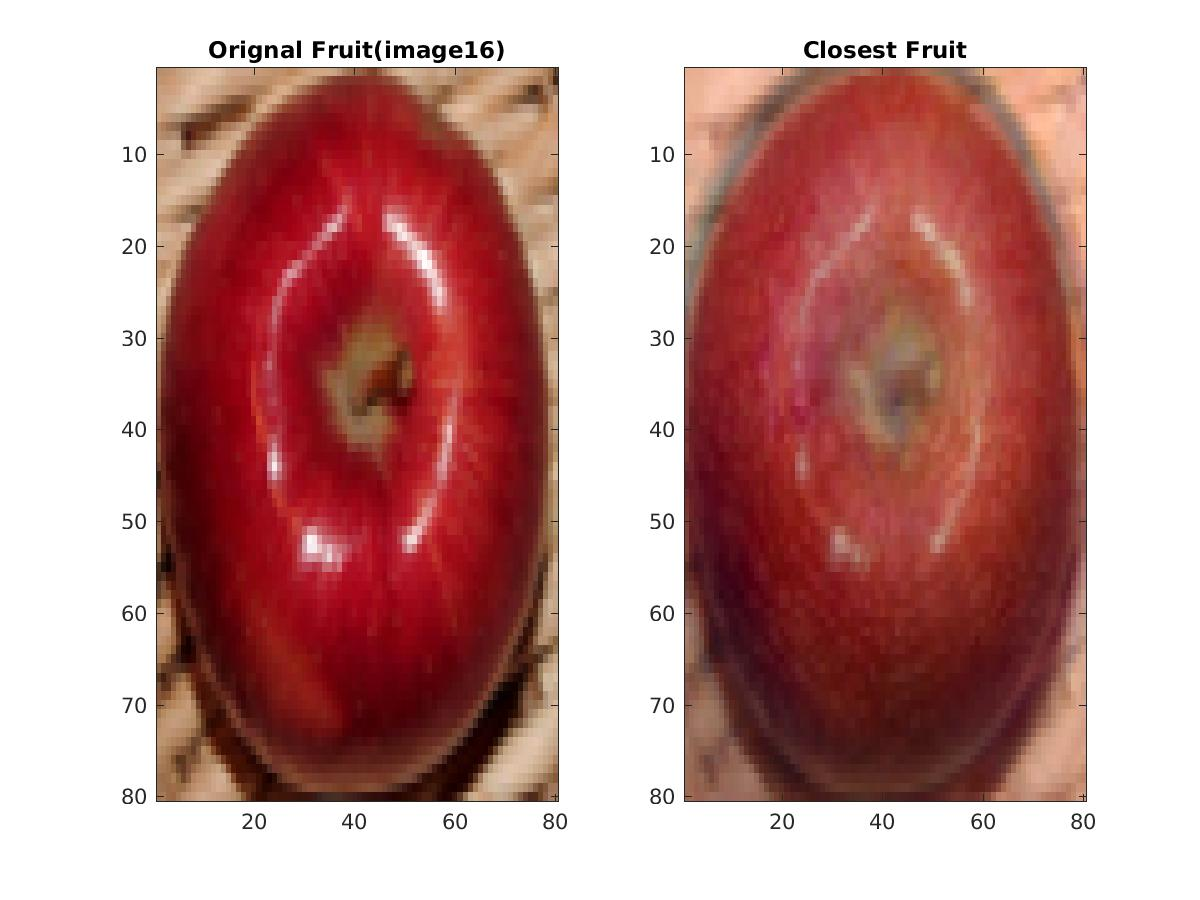
\includegraphics[width=\textwidth, height = 0.25\paperheight]{Closest_fruit_analysis_16}


\newpage
\subsection*{5.3 : Part C}
Now, for generating a new representation of a fruit, let us recall the equation that we started with in Part B. 
$$\boldsymbol{X^i} = \boldsymbol{\mu} + a_1\boldsymbol{V_1} + a_2\boldsymbol{V_2} + a_3\boldsymbol{V_3} + a_4\boldsymbol{V_4}$$
In this case, we need to draw random values of $a_i$ for generating a new fruit. \\ 
We know that the \textbf{magnitude} by which any particular feature varies along an eigenvector is \textbf{proportional} to it's corresponding \textbf{eigenvalue}. \\ Since we are taking the linear combinations of the eigenvectors into the mean to form another image, it would be most suitabe if all the $a_i$ would be the \textbf{corresponding} \textbf{eigenvalues} \\ 
Hence, we have:
$$a_i \in G(\mu=0, \sigma^2 = EigenValue) $$
This was the algorithm that I used to generate new instances of fruits.

 \noindent The plots for the new generated images are as follows.:
 
\noindent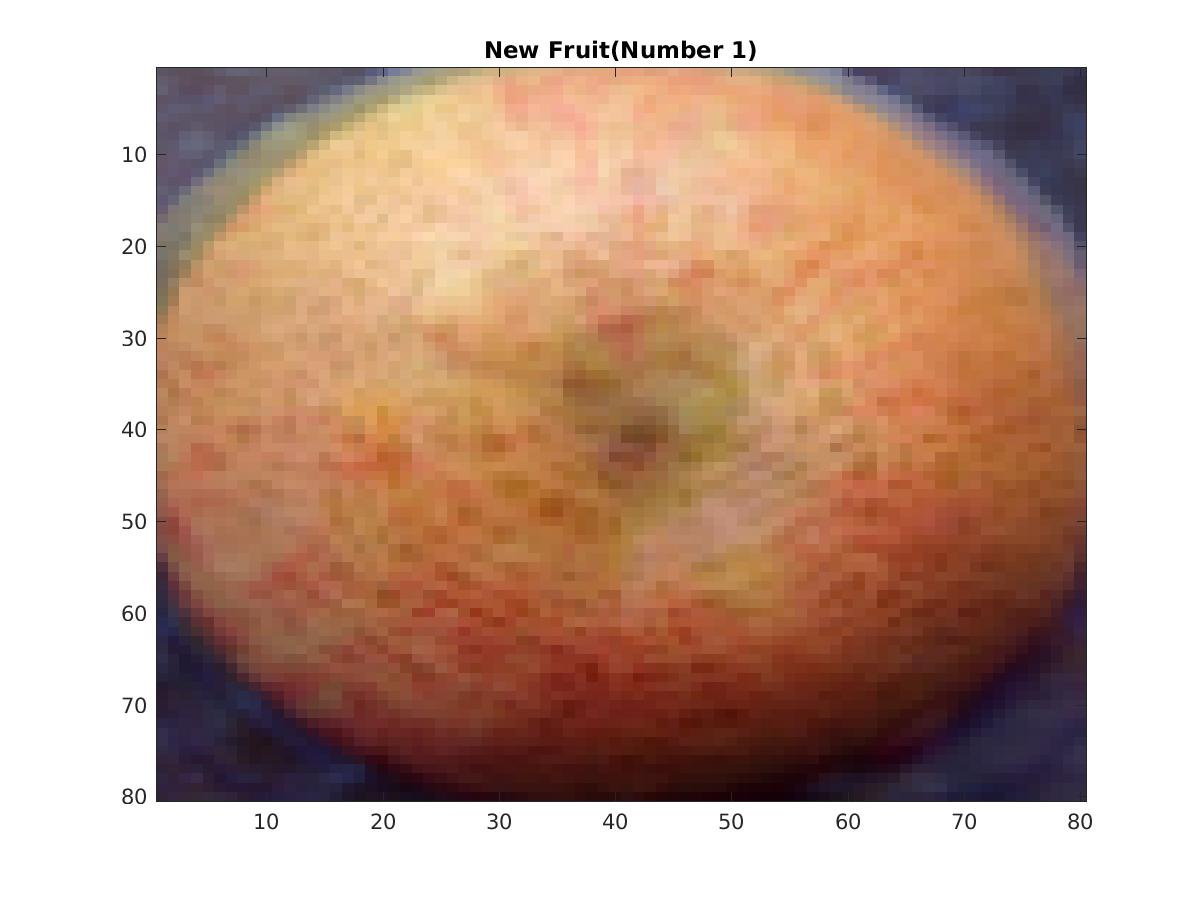
\includegraphics[width=0.7\textwidth, height = 0.25\paperheight]{New_Fruit_Creation_1}\\
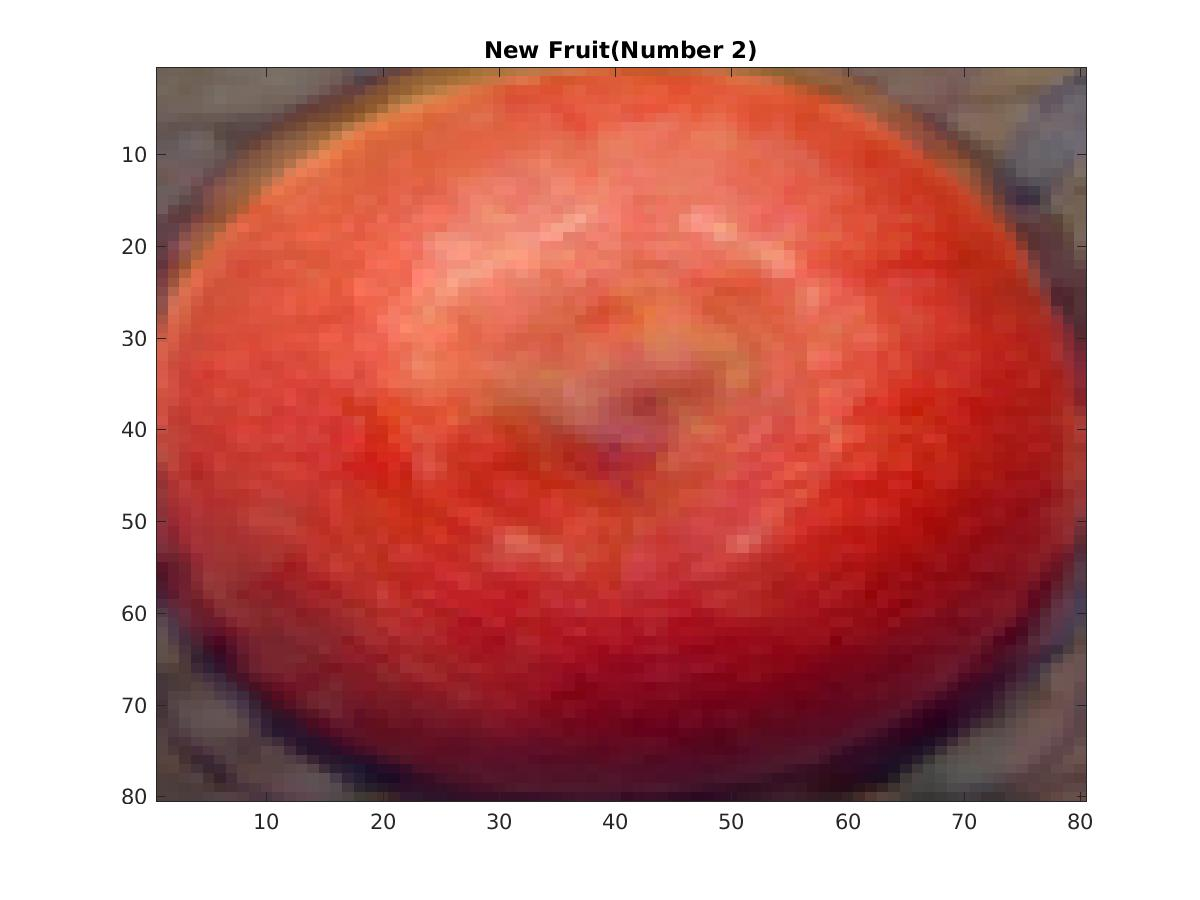
\includegraphics[width=0.7\textwidth, height = 0.25\paperheight]{New_Fruit_Creation_2}\\
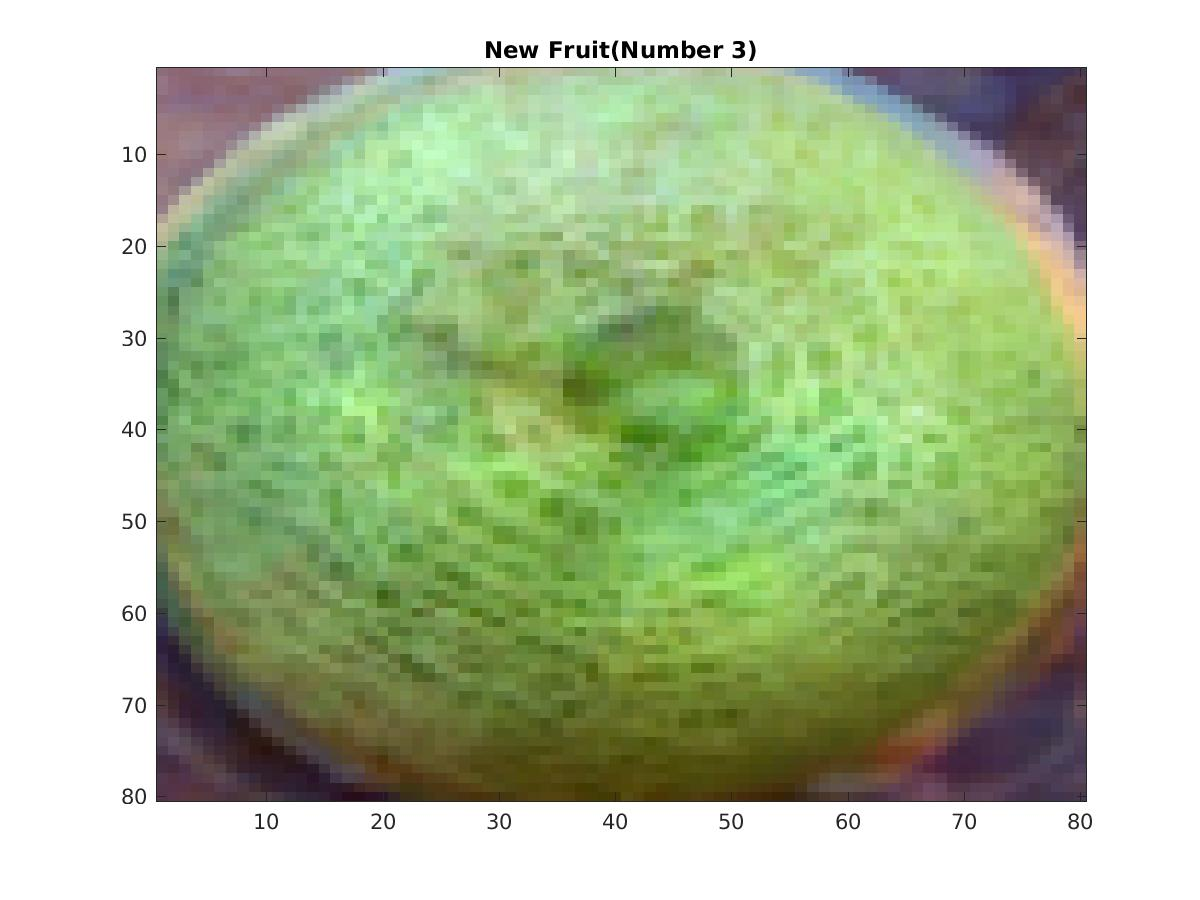
\includegraphics[width=0.7\textwidth, height = 0.25\paperheight]{New_Fruit_Creation_3}\\

\subsection*{5.4 : Usage of Code}
The following are the instructions for the usage of the code:
\begin{itemize}
\item Load the code present in \lq submission/code/q5/q5.m \rq \space.
\item In the same directory are functions implemented like myMean, myCov which return the mean and covariance of appropriate matrices. Functions like myScale, myeigs scale the data and return sorted eigenvalues and eigenvectors, respectively.
\item Simply run the code in \lq q5.m \rq \space and this wil automatically create the required plots. (Requires a lot of time)
\item Lines 39, 44, 63, 81 (commented by default) hava a code to save jpg files of the respective plots. Comment/Uncomment these lines appropriately according to need.
\item The results.mat present in \lq results/mat\rq \space contains all the required results for the partA stored: 
	\begin{description}
	\item[Mean Vector:] Stored as a 19200x1 vector by the name MeanFruit
	\item[Covariance Matrix:] Was not be able to store and upload this file to moodle, since it's a 19200x19200 matrix, and has a whooping size of 2.6 GB.
	\item[Largest 10 EigenVectors:] Stored as a 19200x10 matrix by the name EigenVectors, with each column as a eigenvector.
	\item[Corresponding Eigenvalues:] Stored as a 10x1 vector by the name EigenValues, where the ith cell has the ith largest eigenvalue \lq i\rq
	\end{description}

\end{itemize}
 
\end{document}